\textcolor{black}{\section{Procedimiento}}

\noindent Se construyó un arreglo de 8 LEDs de distintas longitudes de onda ($\lambda$), cada una conectadas a una resistencia de $8.2\,k\Omega$ y de manera independiete (Figura \ref{Foto1}). Posteriormente se armó el circuito de la Figura \ref{Diag1}, con cada uno de los LEDs, de la siguiente manera: se utilizó una fuente de alimentación de corriente directa (CD) UNI-T UDP6721, donde su salida se conectó a la terminal positiva de un multímetro digital Keithley 2110 5.5 para medir la corriente corriente ánodo-cátodo ($I_{A-K}$), por lo que la salida común de este multímetro se conectó a la terminal del LED. Despúes, de un multímetro Steren UNI-T MUL-600, se conectó la terminal roja al punto en el que la resistencia y el ánodo del LED hace contacto, con lo que se pudo medir el voltaje ánodo-cátodo ($V_{U}$). Este montaje se puede observar en la Figura \ref{Foto2}.

\begin{figure}%[H]
	\centering
	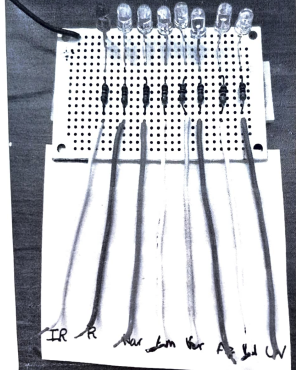
\includegraphics[scale=0.5]{figs/Foto1.png}
	\caption{Acomodo de 8 LEDs conectados a una resistencia de $8.2\,k\Omega$, todos de manera independiente.}
	\label{Foto1}
\end{figure}

\begin{figure}%[H]
	\centering
	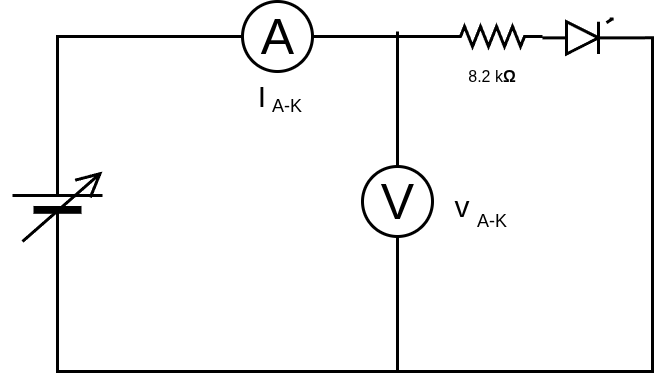
\includegraphics[scale=0.3]{figs/Diag1.png}
	\caption{Circuito para medir la corriente y voltaje de un LED con una resistencia de $8.2\,k\Omega$ conectados a una fuente variable.}
	\label{Diag1}
\end{figure}

\begin{figure}[H]
	\centering
	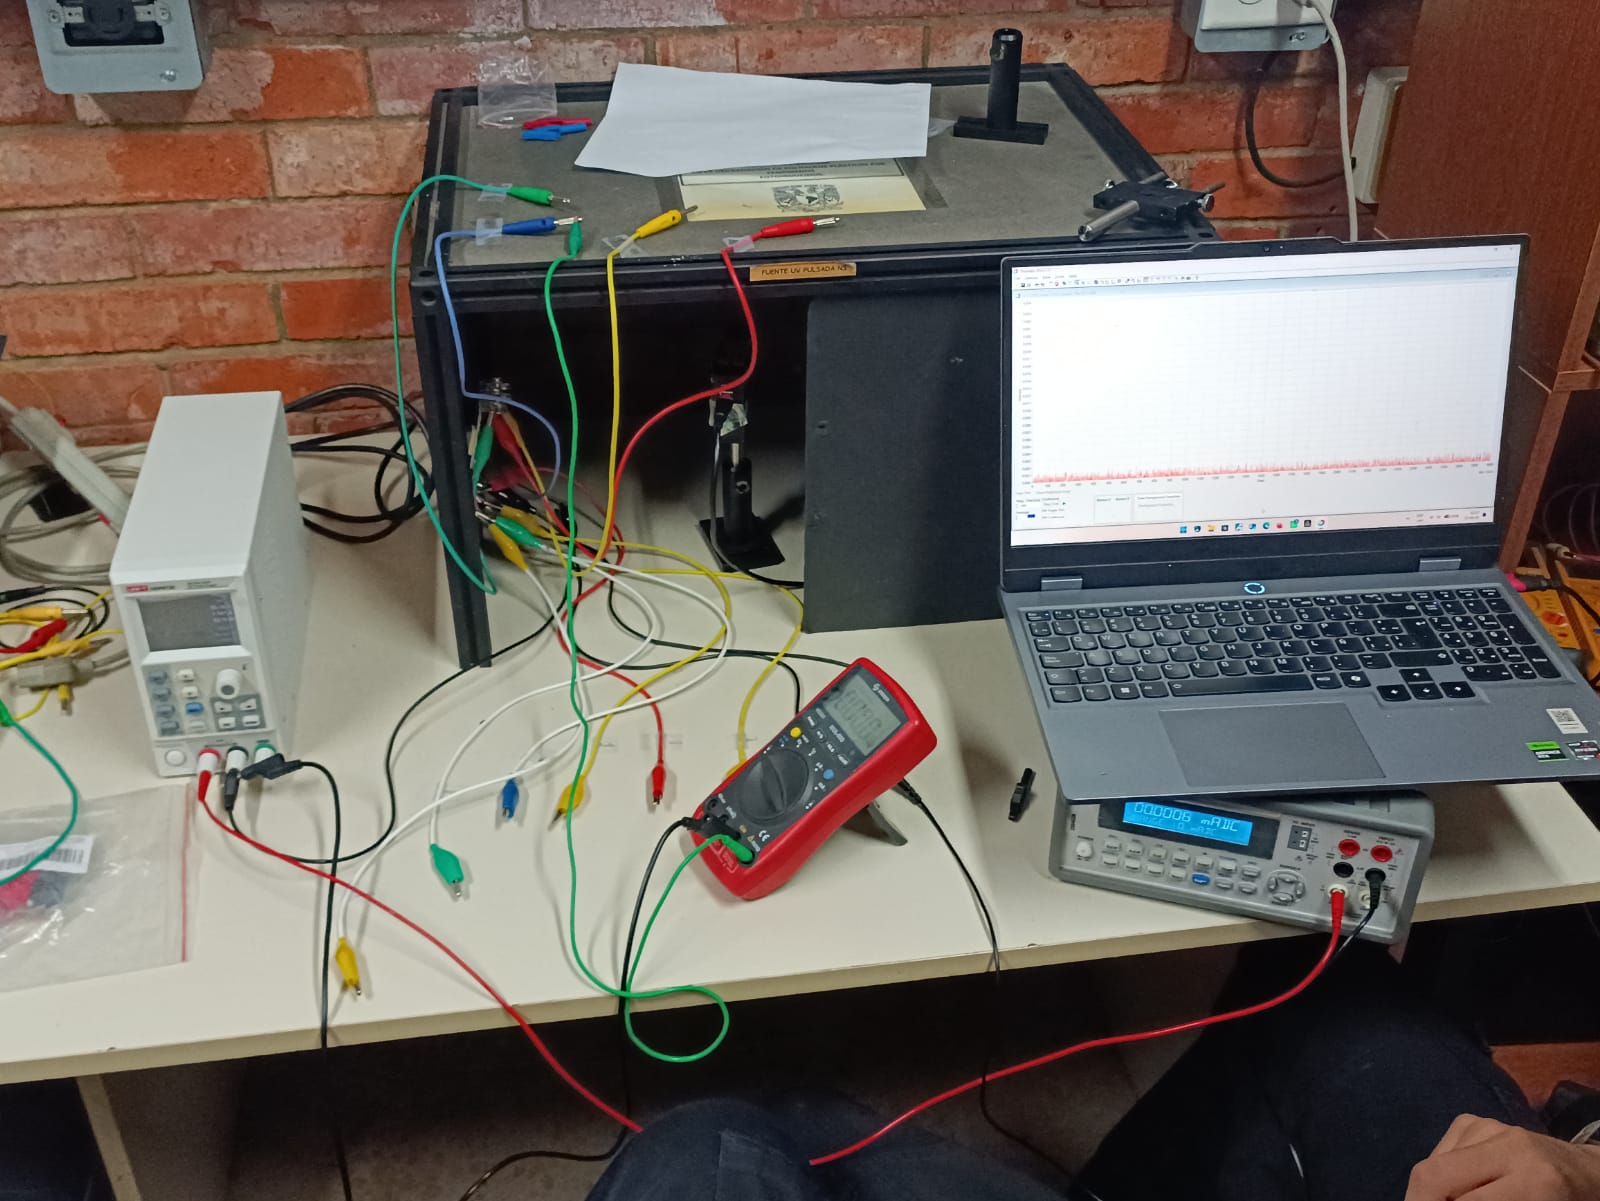
\includegraphics[scale=0.1]{figs/Foto2.jpg}
	\caption{Montaje del circuito para medir la corriente y voltaje de un LED conectado a una fuente variable haciendo uso de una caja negra óptica y una CCD.}
	\label{Foto2}
\end{figure}

Una vez armado el circuito se utilizó una caja negra para óptica para cubrirlo y se colocó un CCD LC1-USB Thorlabs dentro, con el que se midió el espectro del LEDs. Finalmente, se aumentó lentamente el voltaje de salida de la fuente hasta que el LED se encendiera (esto se monitoreó con la CCD), cuidando que la corriente a través del LED se encuentre entre $5$ y $15$ $\mu A$.

Todo el procedimiento se repitió con cada uno de los 8 LEDs y se registraron las mediciones de $V_{U}$ y del espectro correspondiente, para determinar su $\lambda$.